\chapter{МЕТОД STRUCTURE FROM MOTION}

\textbf{Structure from Motion} (дословно \quotes{\textit{структура из движения}}, SFM) - техника построения трёхмерных структур из последовательности двухмерных изображений (фотографий, кадров видео) используемая в области компьютерного зрения. В биологии описывает феномен, позволяющий человеку восстанавливать трёхмерную структуру окружающего мира по двухмерным проекциям на сетчатку глаза.

\section{Основные тереоретические понятия}

Люди с рождения обладают зрением, что позволяет нам распознавать изображения и объекты на них, сравнивать их между собой, оценивать расстояния и размеры. Всё это человеческий мозг делает бессознательно, автоматически. Однако, для машины изображение — всего лишь закодированные данные, набор нулей и единиц. Одной из основных проблем в сопоставлении изображений является очень большая размерность пространства, которое обладает информацией. Если взять маленькую картинку размером хотя бы $100*100$ пикселей, то уже получим количество информации равное $10^4$ пикселей. Поэтому методы анализа изображения должны быть быстрыми и эффективными.

Существует ряд других проблем и сложностей при попытке интерпретации изображений. Одни и те же объекты на разных изображениях могут очень сильно отличаться. На это влияют такие параметры как: точка зрения, освещение (один и тот же объект может быть белым, серым или чёрным в зависимости от освещения), масштаб, деформация и перекрытие объектов, маскировка (слияние с фоном). Поэтому для полноты картины требуется как можно больше различных изображений одного объекта.

\vspace{1em}
Так как же машина обретает зрение?

Основная идея состоит в том, чтобы получить какую-то характеристику, которая будет хорошо описывать изображение, легко вычисляться и для которой можно ввести оператор сравнения. Эта \quotes{характеристика} должна быть устойчива к различным преобразованиям (сдвиг, поворот и масштабирование изображения, изменение яркости, изменение положения камеры). Это необходимо для того, чтобы было возможно определить один и тот же объект на изображениях сделанных с разных углов, расстояний и при разном освещении.

Все эти условия приводят к необходимости выделения на изображении особых, \textit{ключевых точек} (\textbf{key points}). Этот процесс называется \textit{извлечение признаков} (\textbf{feature extraction}). Ключевая точка (локальная особенность) - это такая особая точка, которая достаточно хорошо отличается от близлежащих точек по какой-то определённой характеристике. Она должна быть сильно \quotes{не похожа} на остальные точки вокруг, соответственно может являться, в какой-то степени, уникальным свойством изображения в своей локальной области. Таким образом машина может представить изображение как модель, состоящую из особых точек. Например, на изображении человеческого лица функции ключевых точек могут выполнять глаза, уголки губ, кончик носа.

\vspace{1em}
К особым точкам предъявляются следующие требования:
\begin{enumerate}
    \item Повторяемость (Repeatability). Особенность не должна менять свое положение при изменении точки зрения или освещения;
    \item Значимость (Saliency). Каждая особенность должна иметь уникальное описание;
    \item Компактность (Efficiency). Количество особенностей должно быть существенно меньше числа пикселей изображения;
    \item Локальность (Locality). Особенность должна занимать небольшую область изображения, чтобы снизить вероянтность перекрытия другими объектами.
\end{enumerate}

\vspace{1em}
После выделения особых точек компьютеру нужно уметь их сравнивать (отличать друг от друга). Этот процесс называется \textit{сопоставление признаков} (\textbf{feature matching}). Для сравнения удобно использовать \textit{дескрипторы} (\textbf{descriptor} - \quotes{описатель}). Дескриптор - своеобразный идентификатор ключевой точки, представляющий её в удобном для сравнения и понятном для машины виде. Является вектором, содержащим признаки особой точки. Как мы увидим далее, именно благодаря дескрипторам получается инвариантность относительно преобразований изображений.

\begin{figure}[h]
    \centering
    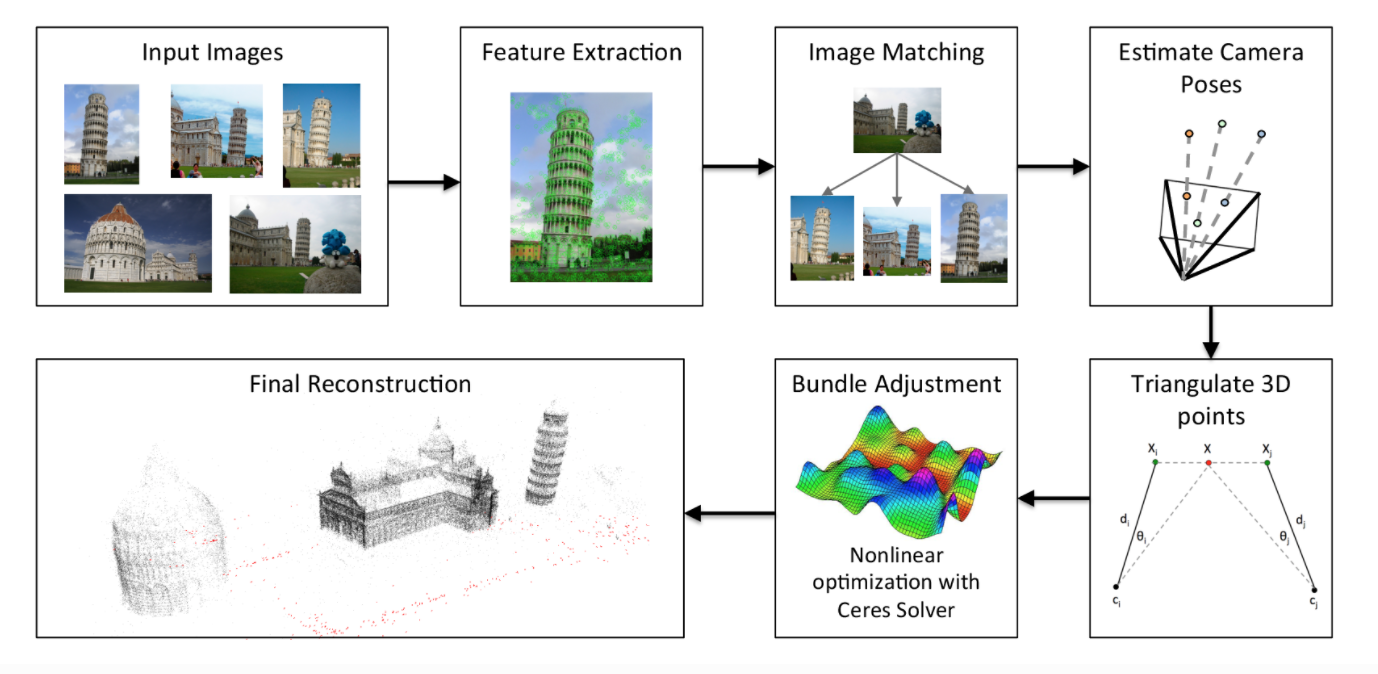
\includegraphics[width=1\textwidth]{sfm.png}
    \caption{\textbf{SFM pipeline}}
    \label{fig:sfm}
\end{figure}

\section{Последовательность шагов процесса SFM}

На рисунке \ref{fig:sfm} представлена схема, демонстрирующая процесс восстановления 3D модели поверхности. 

\vspace{1em}
Можно выделить следующие составляющие процесса реконструкции: 
\begin{enumerate}
    \item Выделение ключевых точек и дескрипторов;
    \item Сравнение дескрипторов и нахождение паросочетаний соответствующих друг другу особых точек;
    \item Нахождение геометрического преобразования, которое переводит ключевые точки одного изображения в соответствующие им точки другого изображения;
    \item Позиционирование камер (изображений) и расположение их в трехмерном пространстве.
\end{enumerate}

\vspace{1em}
Далее будут подробнее рассмотрены описанные выше этапы и используемые на них алгоритмы. Алгоритмы, применяемые на первых двух этапах называют \textit{алгоритмами основанными на особых точках} (\textbf{feature-based algorithms}).
